\documentclass[a4paper,UTF8]{ctexart}

\usepackage{amsmath, amsthm, amssymb, amsfonts, hyperref, mathrsfs}%美国数学学会的包+?
\usepackage{geometry} %控制界面
\usepackage{bookmark}
\usepackage{fancyhdr} % header & footer
\usepackage{appendix} % 附录
\usepackage{tikz} %作图
\usepackage{graphicx} %插入图片的宏包
\usepackage{float} %设置图片浮动位置的宏包
\usepackage{subfigure} %插入多图时用子图显示的宏包
\usepackage{listings} %引用代码
\usepackage{physics,mathtools} %物理数学工具
\geometry{top=2.5cm,bottom=2.5cm,left=2.5cm,right=2.5cm} % 布局要求
\pagestyle{fancy} % fancy分格
\fancyhf{} % 清除所有页眉页脚
\renewcommand\headrulewidth{0.6pt}
\renewcommand\footrulewidth{0.6pt}
\lhead{何金铭 PB21020660}
\chead{座位号:2}
\rhead{\thepage}
\lfoot{2022.9.27}
\rfoot{USTC}
\bibliographystyle{plain} % 引用样式
%============================================================

\begin{document}

\begin{center}
    \textbf{\Large 测量金属丝的杨氏模量和泊松比}
    \par \text{\large 何金铭 PB21020660}
\end{center}

\section{实验目的}
测量金属丝的杨氏模量和泊松比
\section{实验原理}

\subsection{金属丝的杨氏模量和泊松比}
拉力 F 与丝的原始横截面 A 之比定义为应力,伸长量 $\Delta L$
与丝的原始长度 L 之比定义为
纵向线应变。在弹性范围内,应力与应变满足胡克定律:

\begin{equation}
    \frac{F}{A} = E \frac{\Delta L}{L}
\end{equation}

其中 E 为材料的杨氏模量。

横向变化量 $\Delta d$与丝的原始横向长度 d 之比定义为横向线应变。
在材料弹性范围内,横向线应变$\frac{\Delta d}{d}$与纵向线应变$\frac{\Delta L}{L}$之比为常数:

\begin{equation}
    \frac{\Delta d}{d} = -\mu \frac{\Delta L}{L}
\end{equation}

$\mu$为横向变形系数或称泊松比。

\subsection{非平衡电桥}

图 1 为非平衡电桥的原理图,其中电阻箱 $R_1$、$R_2$、$R_3$ 为电桥的三个臂,电阻箱 $R_4$ 与待
测金属丝电阻 $R_s$ 串联构成第四臂,$R_0$ 为电位器,C 是
滑动头。当电桥平衡时:

\begin{equation*}
    \frac{R_1}{R_2} = \frac{R_3}{R_4+R_s}
\end{equation*}

\begin{figure}[!hp]
    \centering
    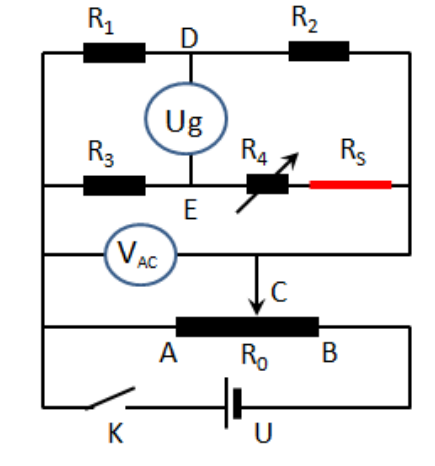
\includegraphics[scale=0.7]{static/fig1.png}
    \caption{非平衡电桥}
\end{figure}

任意桥臂阻值变化时,电桥将偏离平衡位置。金属丝
受到拉伸引起电阻变化$\Delta R_s$,当 $R_4+R_s$ 的相对阻值变化
量小于 1\%时,桥电压 Ug(即 D、E 之间的电压)与该桥臂的电阻变化量近似满
足线性关系:

\begin{equation}
    U_g = \frac{U_{AC}}{4}\cdot \frac{\Delta R_s}{R_4+R_s}
\end{equation}

即将电阻的微小变化量转化成直流电压信号进行测量。

\section{实验仪器}
金属丝(已焊接两根导线),铝支架(已装配电位器、开关、电桥盒等),卷尺(最大允差 2.0mm),
JCD3 型读数显微镜(最大允差 0.015mm),读数显微镜垫块,ZX38A/10 型交直流电阻箱(0.1 级),
KEITHLEY 台式万用表,
直流稳压电源(~1.5V),砝码托盘(配 10 个增砣砝码,每个砝码 100.0g。),导线
\section{实验内容}

1. 利用读数显微镜,测量金属丝的杨氏模量

2. 利用非平衡电桥,测量金属丝的泊松比;

3. 对两个焊点进行哈气,观察 Ug 的变化并进行解释分析。

\section{测量记录}

已知物理量:

1. 每个砝码质量$m = 100g$

2. 金属丝的直径$d = 0.2mm$

\subsection{杨氏模量相关实验数据}

实验中所有开始测量前都放置两个砝码使得托盘稳定。

\begin{table}[!hp]
    \begin{center}
    \begin{tabular}{|c|c|c|}
    \hline
    $l_1/cm$ & $l_2/cm$ & $l_3/cm$ \\
    \hline
    119.81 & 119.80 & 119.65 \\
    \hline
    \end{tabular}
    \end{center}
    \caption{固定线的桩子到靠近重物的焊点的距离记录表}
\end{table}

\begin{table}[!hp]
    \begin{center}
    \begin{tabular}{|c|c|c|c|c|c|c|c|}
    \hline
    \bfseries 放置砝码个数$n$ & 0 & 1 & 2 & 3 & 4 & 5 & 6 \\
    \hline
    \bfseries 焊点的相对位置$l/mm$ & 28.449 & 28.649 & 28.825 & 29.020 & 29.232 & 29.422 & 29.627 \\
    \hline
    \end{tabular}
    \end{center}
    \caption{放置砝码数$n$与焊点相对位置$l$的变化记录表}
\end{table}

\subsection{泊松比相关实验数据}

1. 电桥平衡时,测得$U_{AC} = 0.4009v$

2. 电桥平衡时,测得$R_4 = 16.58 \Omega$

3. 由于测量泊松比时,焊点的相对伸长量应该与测量杨氏模量时的一致,所以在这次实验测量时就没有重新记录焊点的相对伸长量。

\begin{table}[!hp]
    \begin{center}
    \begin{tabular}{|c|c|c|}
    \hline
    $l_1/cm$ & $l_2/cm$ & $l_3/cm$ \\
    \hline
    91.50 & 91.50 & 91.51 \\
    \hline
    \end{tabular}
    \end{center}
    \caption{两个焊点之间的距离记录表}
\end{table}

以下显示的数据是经过分析筛选之后的数据,具体分析可见“分析与讨论”

\begin{table}[!hp]
    \begin{center}
    \begin{tabular}{|c|c|c|c|c|c|}
    \hline
    \bfseries 放置砝码个数$n$ & 0 & 1 & 2 & 3 & 4 \\
    \hline
    \bfseries 电压表示数$U_g/mv$ & -0.015 & -0.037 & -0.059 & -0.084 & -0.099 \\
    \hline
    \bfseries 焊点的相对位置$l/mm$ & 28.449 & 28.649 & 28.825 & 29.020 & 29.232 \\
    \hline
    \end{tabular}
    \end{center}
    \caption{放置砝码数$n$与电压表示数$U_g$的变化记录表}
\end{table}

\section{分析与讨论}

\subsection{杨氏模量实验分析}

\subsubsection{理论分析}
由
\begin{equation*}
    \frac{F}{A} = E \frac{\Delta L}{L}
\end{equation*}
可得
\begin{equation*}
    \frac{nmg}{\pi \cdot \frac{d^2}{4}} = E \frac{\Delta L}{L}
\end{equation*}
最终可得
\begin{equation}
    \Delta L = \frac{4mgL}{\pi d^2 E} n
\end{equation}

可得 $L /m$-$n$图像的斜率为$\frac{4mgL}{\pi d^2 E} \cdot 10^{3}$

\subsubsection{数据处理}

由表一可得固定桩子到焊点的平均距离$L_{average} = \frac{l_1 + l_2 + l_3}{3} = 119.75cm$

由表二可做出$L /m$-$n$图像,并利用最小二乘法来求其斜率k。

\newpage

\begin{figure}[htb]
    \centering
    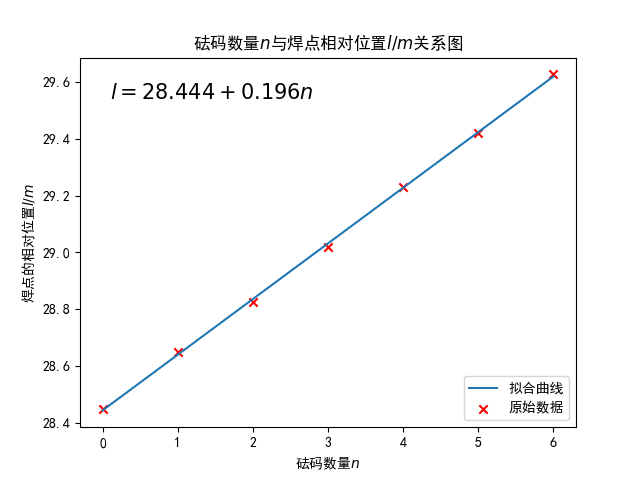
\includegraphics[scale=0.5]{Figure_1.png}
    \caption{$l/m$-$n$图像}
\end{figure}

求得其斜率$k = 0.196 mm$,相关系数$r = 0.9998$

最终得到杨氏模量:

\begin{equation}
    E = \frac{4mgL}{\pi d^2 k} \cdot 10^{3} \\
    = \frac{4 \cdot 0.1 \cdot 9.795 \cdot 1.1975}{\pi \cdot (2 \cdot 10^{-4})^{2} \cdot 0.196} \cdot 10^3 \\
    = 190.491 Gpa
\end{equation}

\subsubsection{误差分析}

计算L的不确定度$U_L$

\begin{equation}
    u_L = \sqrt{\frac{\Sigma^3_{i=1} (l_i-L_{average})^2}{2 \cdot 3}} = 0.05 cm
\end{equation}

\begin{equation}
    u_B = \frac{\sqrt{\Delta^2_{app}+\Delta^2_{est}}}{3} = 0.7 mm
\end{equation}

\begin{equation}
    U_L = \sqrt{(t_p u_L)^2+(k_p u_B)^2} = 0.3 cm
\end{equation}

所以有 $ L = 119.75cm \pm 0.3cm$

计算k的不确定度$U_k$

\begin{equation}
    u_k = k\sqrt{\frac{\frac{1}{r^2}-1}{1\cdot3}} = 0.002 mm
\end{equation}

\begin{equation}
    u_B = \frac{\sqrt{\Delta^2_{app}+\Delta^2_{est}}}{3} = 0.005 mm
\end{equation}

\begin{equation}
    U_k = \sqrt{(t_p u_k)^2+(k_p u_B)^2} = 0.013 mm
\end{equation}

所以有 $k = 0.196mm \pm 0.013mm$

由拓展不确定度得:

\begin{equation}
    \frac{U_E}{E} = \sqrt{(\frac{U_L}{L_{average}})^2+(\frac{U_k}{k})^2} = 0.07
\end{equation}

所以有 $E = 190.491 Gpa \pm 13.334 Gpa$

\subsection{泊松比实验分析}

\subsubsection{理论分析}

联立下式:

\begin{equation*}
    R_s = \rho \frac{L}{A} = \rho \frac{4L}{\pi d^2}
\end{equation*}

\begin{equation*}
    \Delta R_s = \rho \frac{4 \Delta L}{\pi d^2} - \rho \frac{4 L \cdot 2\Delta d}{\pi d^3}
\end{equation*}

\begin{equation*}
    \frac{\Delta d}{d} = -\mu \frac{\Delta L}{L}
\end{equation*}

\begin{equation*}
    U_g = \frac{U_{AC}}{4}\cdot \frac{\Delta R_s}{R_4+R_s}
\end{equation*}

可得:

\begin{equation}
    U_g = \frac{(1+2\mu)R_s U_{AC}}{4(R_4+R_s)L} \cdot \Delta L
\end{equation}

由于拉伸导致$R_s$的变化较小,可以认为$R_s$在拉伸过程中保持不变,$R_s = 51 \Omega - R_4$

可得$\Delta U_g /mv$-$L /mm$图像的斜率的绝对值$|k| = \frac{(1+2\mu)R_s U_{AC}}{4(R_4+R_s)L}$

\subsubsection{数据处理}

由表一可得两焊点间平均距离$L = \frac{l_1 + l_2 + l_3}{3} = 91.503cm$

由表二可做出$\Delta U_g /mv$-$L /mm$图像,并利用最小二乘法来求其斜率的绝对值|k|。

\begin{figure}[!htb]
    \centering
    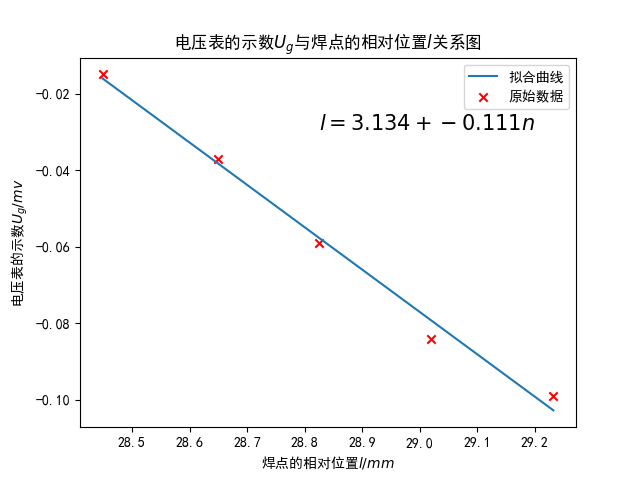
\includegraphics[scale=0.5]{Figure_2.png}
    \caption{$U_g$-$l$图像}
\end{figure}

得$\Delta U_g /mv$-$L /mm$图像的斜率的绝对值$|k| = 0.111$,相关系数$r = 0.997$

由公式六可推得:

\begin{equation}
    \mu = \frac{4(R_4+R_s)L|k|}{2 R_s U_{AC}} - \frac{1}{2} = \frac{4 \cdot 51 \cdot 0.915 \cdot 0.111}{2 \cdot (51 - 16.58) \cdot 0.4009} - \frac{1}{2} = 0.251
\end{equation}

\subsubsection{误差分析}

计算L的不确定度$U_L$

\begin{equation}
    u_L = \sqrt{\frac{\Sigma^3_{i=1} (l_i-L_{average})^2}{2 \cdot 3}} = 0.02 cm
\end{equation}

\begin{equation}
    u_B = \frac{\sqrt{\Delta^2_{app}+\Delta^2_{est}}}{3} = 0.7 mm
\end{equation}

\begin{equation}
    U_L = \sqrt{(t_p u_L)^2+(k_p u_B)^2} = 0.2 cm
\end{equation}

所以有 $ L = 91.503cm \pm 0.2cm$

\begin{equation}
    u_k = k\sqrt{\frac{\frac{1}{r^2}-1}{1\cdot3}} = 0.005 mm
\end{equation}

\begin{equation}
    u_B = \frac{\sqrt{\Delta^2_{app}+\Delta^2_{est}}}{3} = 0.005 mm
\end{equation}

\begin{equation}
    U_k = \sqrt{(t_p u_k)^2+(k_p u_B)^2} = 0.02 mm
\end{equation}

所以有 $k = 0.111mm \pm 0.02mm$

\begin{equation}
    \frac{U_{\mu}}{\mu} = \sqrt{(\frac{U_L}{L_{average}})^2+(\frac{U_k}{k})^2} = 0.18
\end{equation}

所以有 $\mu = 0.251 \pm 0.045$

\subsection{关于记录的实验数据的思考及分析误差来源}

杨氏模量相关的实验数据在上面已经全部给出。

泊松比测量的完整的实验数据如下:

\begin{table}[!hp]
    \begin{center}
    \begin{tabular}{|c|c|c|c|c|c|c|c|}
    \hline
    \bfseries 放置砝码个数$n$ & 0 & 1 & 2 & 3 & 4 & 5 & 6 \\
    \hline
    \bfseries 第一次电压表示数$U_g/mv$ & 0.011 & 0.183 & 0.217 & 0.288 & 0.358 & 0.343 & 0.277 \\
    \hline
    \bfseries 第二次电压表示数$U_g/mv$ & -0.015 & -0.037 & -0.059 & -0.084 & -0.099 & -0.161 & -0.231\\
    \hline
    \bfseries 第三次电压表示数$U_g/mv$ & -0.002 & -0.013 & -0.068 & -0.222 & -0.276 & -0.372 & -0.463 \\
    \hline
    \end{tabular}
    \end{center}
    \caption{放置砝码数$n$与电压表示数$U_g$的变化记录表}
\end{table}

将实验数据做成表格的形式

\newpage

\begin{figure}[!htb]
    \centering
    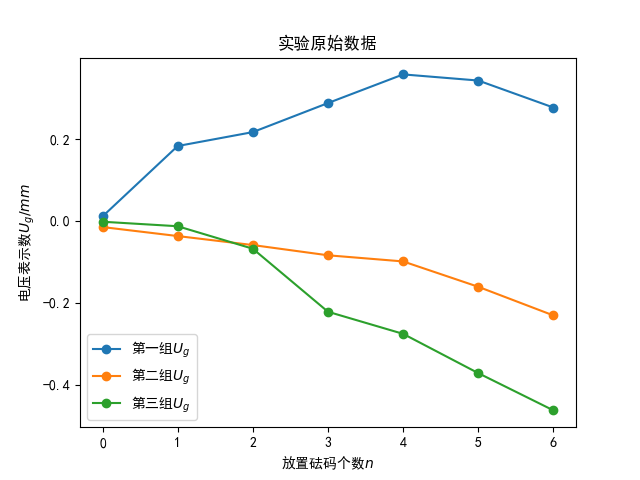
\includegraphics[scale=0.5]{Figure_3.png}
    \caption{原始实验数据}
\end{figure}

第一组实验电压表示数$U_g$偏大可能的原因是刚开始做实验的时候,接完电路之后没有预热15min,仪器没有到达稳定的工作温度,
导致示数偏大;而在第五次测量的时候又开始下降,可能是因为装置已经预热完成,读数恢复稳定。

第二组的实验数据在第一次测量和第五次测量的数据斜率很小,之后的斜率突然变大,可能是因为放置砝码的时候误触碰了托盘,导致托盘带动金属丝的,使其电阻变化。
又观察到第五次测量和第六次测量的数据是线性的,推测也可能是系统产生的变化导致的。

观察三组的数据,发现每族的第五次测量和第六次测量的数据变化的斜率相同,推测可能是因为当托盘中有了六个砝码的时候,金属丝的力学性质发生了改变。

第三的实验数据前三个较为正常,斜率较小,之后的斜率也突然变大,可能是因为第二组中的原因,
也可能是金属丝疲劳,导致示数变大。

综上所述,可能的原因有:

1. 测量电压表示数之前忘记对装置预热,导致示数不稳定

2. 放置砝码时容易触碰到托盘,带动线一起运动,使电阻发生极大的变化

3. 金属丝容易出现疲劳状态,导致电压表示数非完全线性变化

4. 金属丝极易受外界的干扰,比如实验室内其他同学的扰动可能会振动金属丝,空调风容易导致托盘做圆周摆运动

5. 某些装置的焊点可能出现了虚焊的现象

\section{思考题}

观察发现:在远离砝码的焊点哈气的时候,原来已达平衡的电桥示数会先变大、后变小;在靠近砝码的焊点哈气的时候,原来已达平衡的电桥示数会先变小、后变大。

思考:单个示数变化的方向不是关键,而向两个焊点哈气时电压表示数朝两个相反的方向变化才是关键。因为调换电压表的接入方向就可以改变电压表的示数方向。

可能的原因:可能是因为热电偶效应导致这种现象的发生。哈气时容易发生温度的变化,当哈气时可能会产生温差电势,精度较高的电压表可以显示出来;而之后又马上恢复原状,应该是温度马上又恢复室温,电势消失。
两边焊点哈气不对称的结果应该是电势差的空间不对称性造成的。

\end{document}